\chapter{実験}
\label{chap:ex}

%----------------------------------------------
\section{まえがき}
%----------------------------------------------
前章で提案したDNNに基づくパーミュテーション解決法の有効性を確認するために,FDICAで分離した信号を模倣した行列と実際の音声ファイルを用意し,提案パーミュテーション解決法を適用する.後に,その性能を評価した.
\ref{sec:ex_condition}節では,本実験における条件を詳細に示し,\ref{sec:ex_res}節では提案手法のパーミュテーション解決性能を示している.
\ref{sec:matome}節で本章のまとめを述べる.
%----------------------------------------------
\section{実験条件}
\label{sec:ex_condition}
%----------------------------------------------
% \begin{table}[t]
% \begin{center}
%  \caption{Experimental conditions}
%  \label{table:ex}
%   \begin{tabular}{clll}\hline \hline
%    Window function in STFT & Hamming window  \\ \hline
%    Window length in STFT & 512~ms  \\ \hline
%    Shift length in STFT & 128~ms \\ \hline
%    Paramaters in Adam optimizer & \begin{tabular}{c}
%    \begin{flushleft}Learning rate = $0.001$\end{flushleft}\\
%    \begin{flushleft}$\beta = 0.9$\end{flushleft}
%    \end{tabular}  \\ \hline 
%    Reverberation time & $T_{60} = 470$~ms\\ \hline
%    Source direction of training data & $(\theta_1, \theta_2)=(60^\circ, 120^\circ)$\\ \hline
%    Source direction of test data & \begin{tabular}{c}
%    \begin{flushleft}(\theta_1, \theta_2)=(60^\circ, 120^\circ)\end{flushleft}\\ 
%    \begin{flushleft}(\theta_1, \theta_2)=(60^\circ, 100^\circ)\end{flushleft}\\ 
%    \begin{flushleft}(\theta_1, \theta_2)=(70^\circ, 110^\circ)\end{flushleft}
%    \end{tabular}\\ \hline \hline
%   \end{tabular}
%  \end{center}
% \end{table}

\begin{table}[t]
\begin{center}
 \caption{Speech sources obtained from SiSEC2011}
 \label{table:wav}
  \begin{tabular}{clll}\hline \hline
   Signal & Language & Data name &Length~[s]  \\ \hline
   Speech & English & dev3\_female4\_src\_2 & 10.0  \\ \hline
   Speech & English & dev2\_male4\_src\_2 &  10.0 \\ \hline
   \hline
  \end{tabular}
 \end{center}
\end{table}

本実験では,提案するDNNに基づくパーミュテーション解決法において,どの程度各周波数成分の並び替えができるかを実験的に確認した.
実験データとして,全ての成分が0と1の行列,25列毎に0と1の値が入れ替わる行列,1列毎に0と1の値が入れ替わる行列の3パターンを使用した.行列のサイズは全て100行100列とした.
また,ブロックパーミュテーションと呼ばれる,ブロック単位で音源分離に失敗することをふまえ,2行,4行,8行ごとに各周波数成分をシャッフルした実験も同時に実施した.
1列毎に0と1の値が入れ替わる行列に対しては,95\%の割合で1行ごとにシャッフルしそれ以外は2行ごとにシャッフルした場合と,99\%の割合で1行ごとにシャッフルしそれ以外は2行ごとにシャッフルした場合の実験も行った.
加えて,実際の音声信号に対して提案手法がどの程度適用できるかを調べるために,Table~\ref{table:wav}に示すようにSiSEC2011~\cite{Sisec}の英語の音声信号(男性1名及び女性1名)2種類を使用した.
音声信号に対するSTFTは,fftサイズ2048~ms,シフトサイズ1024~msに設定した.また,音声データに対しては8行ごとにシャッフルした場合と16行ごとにシャッフルした場合の2種類の実験を行った.
学習データには,完全分離信号$\bm{Z}_1$と$\bm{Z}_2$の各周波数成分をランダムでシャッフルしたものを用いた.
検証データには学習データにはないシャッフルパターンを用いて$\bm{Z}_1$と$\bm{Z}_2$の各周波数成分をシャッフルさせることで作成した.
DNNの最適化法にはAdam\cite{adam}を用い,ハイパーパラメータはそれぞれ$\varepsilon=1.0\times10^{-8},~\beta_1 = 0.9,~\beta_2 = 0.999$及び学習率$\eta=0.001$とした.
その他の学習パラメータについては,バッチサイズを8,エポック数を1000,学習に用いるシャッフルパターンを300として誤差逆伝搬学習を行った.
主観評価として,各周波数成分において正しく並び替えを行う割合,即ち検証データに対する正答率を用いる.


%----------------------------------------------
\section{実験結果}
\label{sec:ex_res}
%----------------------------------------------

%%%%%%%%%%%%%%%%%%%%%%%%%%%%
\begin{figure}[t]
    \begin{center}
        \includegraphics[width=1.0\columnwidth]{figures/main_01mat_graph.pdf}
    \end{center}
    \vspace{-8pt}
	\caption{Accuracy curves of DNN for training and validation with datasets of a matrix with only zeros and a matrix with only ones.}
	\label{fig:accu_01mat}
\end{figure}
%%%%%%%%%%%%%%%%%%%%%%%%%%%%

%%%%%%%%%%%%%%%%%%%%%%%%%%%%
\begin{figure}[t]
    \begin{center}
        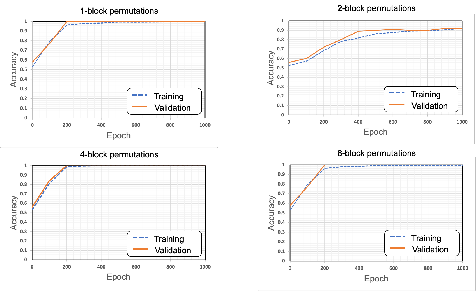
\includegraphics[width=1.0\columnwidth]{figures/SVGgraph_25stripe.pdf}
    \end{center}
    \vspace{-8pt}
	\caption{Accuracy curves of DNN for training and validation with datasets of two matrices with 0 and 1 values swapped every 25 columns.}
	\label{fig:accu_25stripe}
\end{figure}
%%%%%%%%%%%%%%%%%%%%%%%%%%%%

%%%%%%%%%%%%%%%%%%%%%%%%%%%%
\begin{figure}[t]
    \begin{center}
        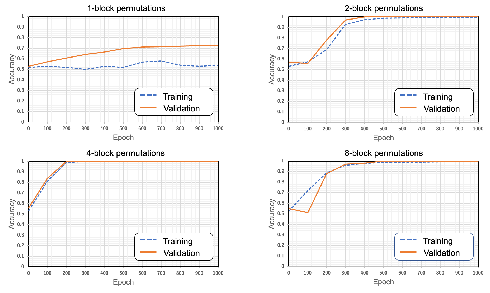
\includegraphics[width=1.00\columnwidth]{figures/SVGstripe_graph.pdf}
    \end{center}
    \vspace{-8pt}
	\caption{Accuracy curves of DNN for training and validation with datasets of two matrices with 0 and 1 values swapped per column.}
	\label{fig:accu_stripe}
\end{figure}
%%%%%%%%%%%%%%%%%%%%%%%%%%%%

%%%%%%%%%%%%%%%%%%%%%%%%%%%%
\begin{figure}[t]
    \begin{center}
        \includegraphics[width=0.8\columnwidth]{figures/graph_stripe_1block99ratio.pdf}
    \end{center}
    \vspace{-8pt}
	\caption{Accuracy curves of DNN for training and validation with datasets of two matrices with 0 and 1 values swapped in each column with a 1\% probability of shuffling two rows together and the rest shuffled row by row.}
	\label{fig:accu_stripe_1block99ratio}
\end{figure}
%%%%%%%%%%%%%%%%%%%%%%%%%%%%

%%%%%%%%%%%%%%%%%%%%%%%%%%%%
\begin{figure}[t]
    \begin{center}
        \includegraphics[width=0.8\columnwidth]{figures/graph_stripe_1block95ratio.pdf}
    \end{center}
    \vspace{-8pt}
	\caption{Accuracy curves of DNN for training and validation with datasets of two matrices with 0 and 1 values swapped per column with a 5\% probability of shuffling two rows together and the rest shuffled row by row.}
	\label{fig:accu_stripe_1block95ratio}
\end{figure}
%%%%%%%%%%%%%%%%%%%%%%%%%%%%

%%%%%%%%%%%%%%%%%%%%%%%%%%%%
\begin{figure}[t]
    \begin{center}
        \includegraphics[width=0.8\columnwidth]{figures/inkscape_graph_audio_8block.pdf}
    \end{center}
    \vspace{-8pt}
	\caption{Accuracy curves of DNN for training and validation with datasets of audio data shuffled into groups of 8 lines each.}
	\label{fig:accu_audio_8block}
\end{figure}
%%%%%%%%%%%%%%%%%%%%%%%%%%%%

%%%%%%%%%%%%%%%%%%%%%%%%%%%%
\begin{figure}[t]
    \begin{center}
        \includegraphics[width=0.8\columnwidth]{figures/inkscape_graph_audio_16block.pdf}
    \end{center}
    \vspace{-8pt}
	\caption{Accuracy curves of DNN for training and validation with datasets of audio data shuffled into groups of 16 lines each.}
	\label{fig:accu_audio_16block}
\end{figure}
%%%%%%%%%%%%%%%%%%%%%%%%%%%%


Fig.~\ref{fig:accu_01mat}〜Fig.~\ref{fig:accu_stripe}には,全ての成分が0と1の行列,25列毎に0と1の値が入れ替わる行列,1列毎に0と1の値が入れ替わる行列の周波数成分に対して
それぞれ1行,2行,4行,8行分をまとめてシャッフルを行った時の結果を示す.この結果から,各周波数成分の8行分をまとめてシャッフルした場合,実験を行った全てのパターンにおいてどれも正答率が100\%に近い値となっている.
しかし,1列毎に0と1の値が入れ替わる行列に対して各行ごとにシャッフルを行った場合は,正答率が54\%程度となった.即ち,提案手法において各行ごとにシャッフルを行なった行列に対してはパーミュテーション問題を解決することが難しいが,ブロック単位でのパーミュテーション問題は容易に解けると言える.
Fig.~\ref{fig:accu_stripe_1block99ratio}とFig.~\ref{fig:accu_stripe_1block95ratio}より,1列毎に0と1の値が入れ替わる行列に対して,95\%の割合で1行ごとにシャッフルしそれ以外は2行ごとにシャッフルした場合の正答率は93\%程度となったが,99\%の割合で1行ごとシャッフルしそれ以外は2行ごとにシャッフルした場合の正答率は60\%程度となった.
このことより,DNNは少しでもブロック単位でシャッフルが行われていると学習が容易となることがわかる.
Fig.~\ref{fig:accu_audio_8block}とFig.~\ref{fig:accu_audio_16block}より,音声データに対して8行ごとと16行ごとのブロック単位でのパーミュテーション問題として考え実験を行った結果,どちらのグラフでも正答率が80\%を超えた.



\clearpage




\clearpage
%----------------------------------------------
\section{本章のまとめ}
\label{sec:matome}
%----------------------------------------------
本章では,提案手法の有効性を確認するため,FDICAを適用した後のパーミュテーション行列を模倣した人工データと実際の音声データを用いて,実験を行った.
実験の結果より,人工データを用いたブロック単位でのパーミュテーション問題に対しては,どのような行列であっても100\%に近い確率で解決できることを示した.
実際の音声データに対しても,ブロック単位でシャッフルが行われていると80\%を超える正答率になることを示した.
次章では,本論文における総括とした結論を述べる.
